\section{Introduction}
Medical Errors characterized by adverse events due to human and system factors
(as opposed to diseases) are the third leading cause of mortality in the United
States. Referred to as Preventable Medical Errors (\PME{}), they are defined as
incorrect intended treatment, or incorrect executions of intended treatment
\cite{DonaldsonBook00}.
To mitigate such errors, hospitals and Medical Associations publish
evidence-based statements that codify recommended best practice for
various scenarios called Best Practice Guidelines (\BPGs{}) \cite{field1990clinical}.
\BPGs{} are routinely updated based on results from clinical trials and advances in medical science,
providing Healthcare Professionals (\HCPs{}) with the latest diagnosis and treatment related information.

\BPGs{} can only be effective at reducing \PMEs{} if \HCPs{} adhere to them.
For example, consider Advanced Cardiac Life Support (\ACLS{}): a \BPG{} published
by the American Heart Association (AHA) for management
of In Hospital Cardiac Arrest (IHCA): a life-threatening condition \cite{AHAGuidelineAdult, AHAGuidelinePed}.
Studies suggest that management
of IHCA in 30\% of adult, and 17\% of pediatric cases deviates from the
AHA-prescribed \BPG, resulting in worse patient outcomes \cite{Ornato2012DeviationAdult,Wolfe2020DeviationPediatric,
Crowley2020DeviationAdult,Honarmand2018Adherence,Mcevoy2014Adherence}.
Thus, ensuring \BPG{}-adherence is vital. However, it has been shown that
having clinicians adhere to \BPGs{} is difficult to achieve in practice
\cite{RandJAMA99,DavisCMAJ97}. To address this, computerized Decision Support Systems that codify \BPGs{} and supports \HCPs{} with
situation-specific advice, called Clinical Guidance Systems (\CGSs{}), can be utilized.
Such systems have demonstrated effectiveness at improving \BPG{} adherence
\cite{KwokEMA09}. Moreover, evidence from multi-center clinical trials
suggests that such systems are effective at reducing \PMEs{} \cite{BenettJAMIA16,SahotaJIS11}.

We briefly provide an overview of existing research on \CGSs{} to explain why
it doesn't addressed problems we intend to address in this proposal.
There exists a large body of research on \CGSs{}. In
\cite{PelegJBI13}, the author provides a methodological review of
existing work on Computer Interpretable Guidelines (\CIGs{}): executable
formalizations of \BPGs{} used to construct \CGSs{}.
Existing work is classified into one of eight themes spanning
the entire development cycle of a \CIG{}. The themes and relations between them
are shown in \figurename{} \ref{fig:cpg-research-topics}.

\begin{wrapfigure}{l}{0.5\textwidth}
  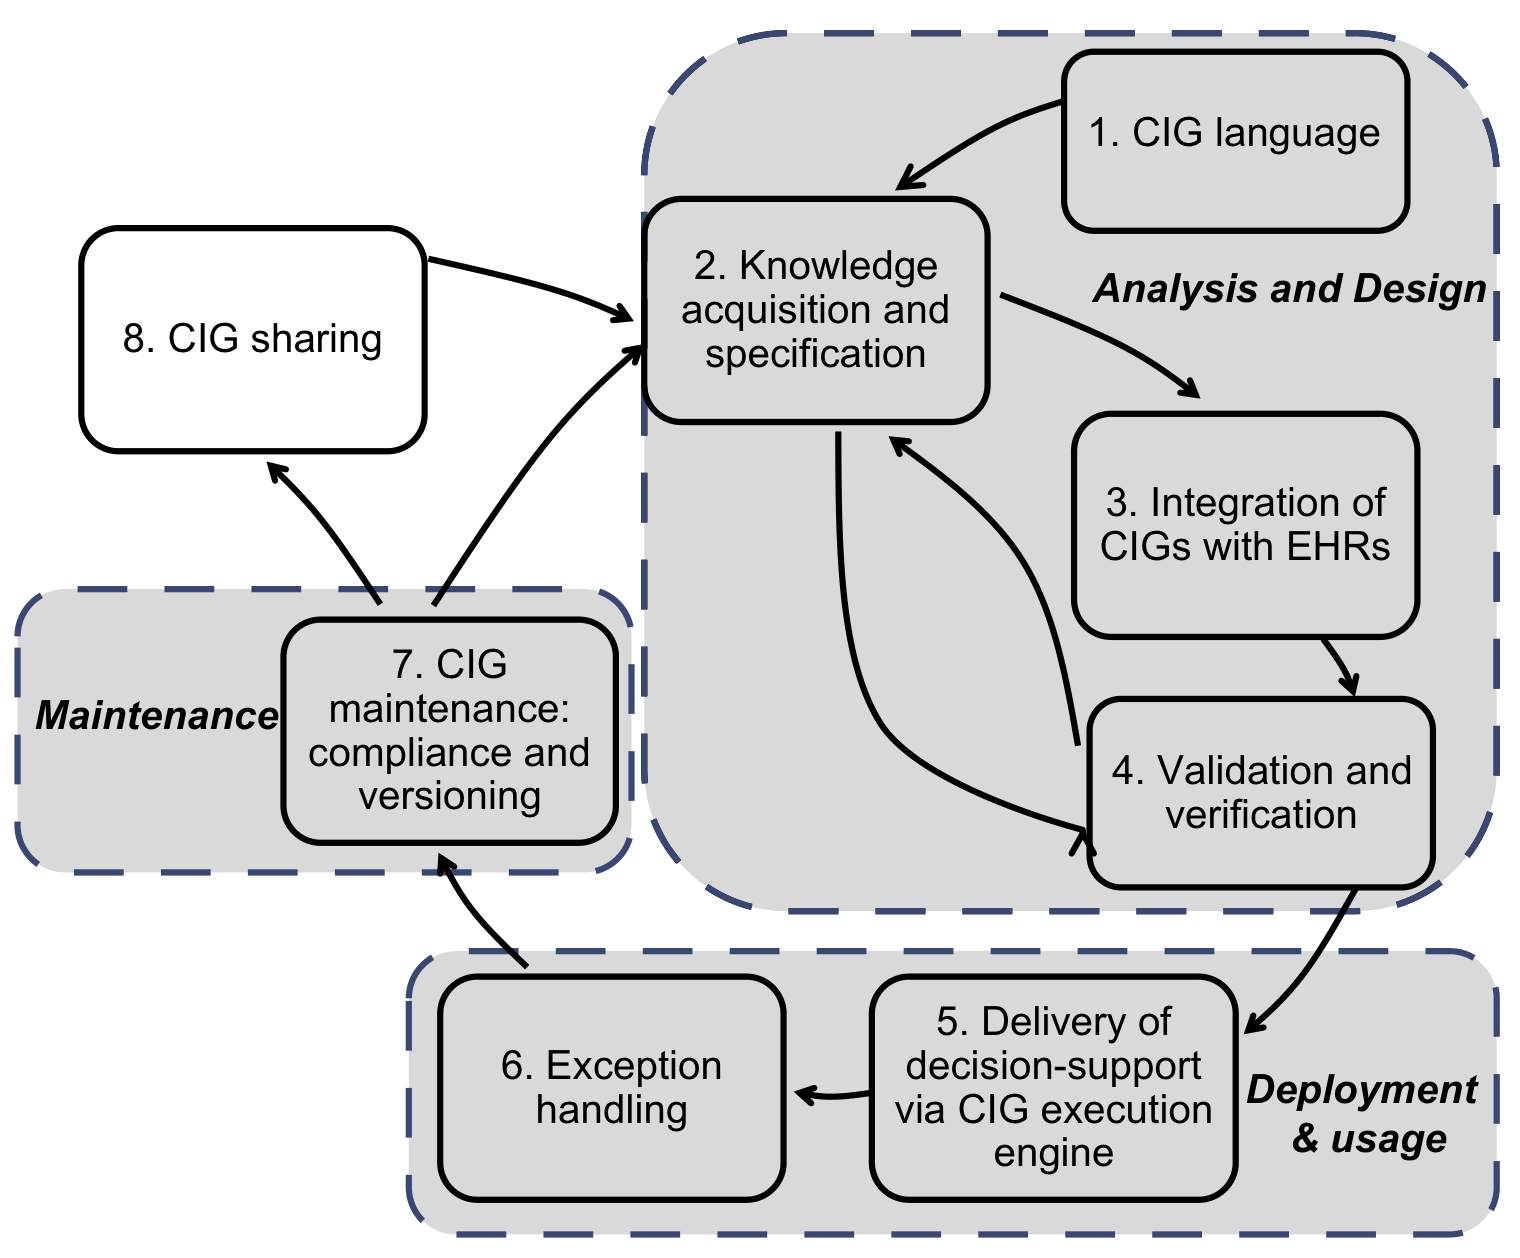
\includegraphics[width=\linewidth]{cpg-topics}
  \caption{\CGSs{} Research Themes}\label{fig:cpg-research-topics}
\end{wrapfigure}

According to the author in \cite{PelegJBI13}, \CIGs{} are usually based on previously published non-executable
\BPGs{}. To develop a \CIG{}, a language is identified in (1). Teams of
software developers and clinicians then collaborate to express medical knowledge
in the \BPG{} in the identified language. In (3), the \CIG{}
is integrated with components such as a Graphical User
Interface (\GUI{}), Electronic Health Records (\EHRs{}) and external devices
(such as monitors for patient parameters) to obtain a \CGS. Before adoption
in the real-world, it is imperative to ensure that the \CIG{} \emph{mirrors}
the underlying \BPG{}. This validation occurs by \emph{testing} the \CGS{}
using execution capabilities of the modeling language from (1) in (5).
Additionally, formal verification may be used to establish other desired
properties hold. Inconsistencies identified in (5) are fixed through developer-clinician
collobaration in (2),  re-validation and
verification. While the aforementioned development cycle has resulted in several
effective \CGSs{}, it has some limitations:

\paragraph{Gap between specification and implementation:}

To develop the \CIG{}, software developers rely on clinicians to interpret the
non-executable \BPG{} and communicate
the intended semantics to them. Thus, the non-executable \BPG{} serves as a functional specification for
the \CIG{}, i.e. the implementation. In such safety-critical systems, it is
imperative that the implementation, i.e. the \CIG{}, conforms to its
specification, i.e., the \BPG{}. To address this, the \CIG{} is tested by
putting the \CGS{} through clinical simulations. But, while testing reduces
the risk of non-conformance, it does not completely eliminate it.

\paragraph{Safe Modularity:}

While developing \CGSs{} is both complex and cost-intensive,
the development effort can be reduced by sharing \CGSs{} across hospitals \cite{PelegAMIA00}.
But, even for the same \BPG{}, hospitals develop their own \CGSs{} to address
their needs, resulting in duplicated work.
For instance, for the \ACLS{} \BPG{}, multiple \CGSs{} have been developed by different
different hospitals in a span of just six years years \cite{FullCodePro,PediAppRREST2020,
PediAppRREST2021,GuidingPad2017,GuidingPad2019, GuidingPad2020,DST2014,DST2019,ROSCo2021,TeamScreen2019,Wu2017}.
\CGSs{} based on the same \BPG{} typically have the same \CIG{}, but may differ
in their Graphical User Interfaces (\GUIs), or integration with external
devices, to address hospital-specific needs.
To enable safe sharing of knowledge, we need a mechanism that:
\begin{enumerate*}[label=(\alph*)]
  \item allows a stable, formally-verfied \CIG{} that is \emph{decoupled} from other
    components, and,
  \item supports hospital-specific customizations without compromising system
    \emph{safety}.
\end{enumerate*}

\paragraph{Holistic System Safety:}

Actions performed by a \CGS{} can either be \emph{programming-oriented}
or \emph{clinically-oriented} \cite{BoxwalaJBI04}. \emph{programming-oriented}
actions are peformed by executing the \CIG{} itself. For example,
using patient parameters, or health records to make a reccomendation or diagnosis,
or to raise a warning. \emph{clinically-oriented} actions on the other hand
are ones that involve a clinician. For example, in the case of \ACLS{},
the \CGS{} recommends that Cardiopulmonary Resuscitation (\CPR{}) be performed
for a certain length of time. Such actions can only be performed by clinicians,
an the \CGS{} assumes that the recommended action was indeed performed before
moving resuming guidance.

For holistic system safety, both categories of actions must be completed
successfully. While traditional formal reasoning techniques can be employed
to establish correctness of \emph{programming-oriented} actions, the same
cannot be used to reason about \emph{clinically-oriented} ones.
Thus, a mechanism that allows some guarantees about clinically-oriented is
desirable.


\paragraph{Formal Semantics:}

Since \CIGs{} are safety-critical, it is vital that the
language in which they're developed has complete formal semantics that
can be used to derive tools such as semantically-correct interpreters,
deductive program verifiers, and model-checkers.

\subsection{Limitations of Existing Approaches}

While existing approaches have been imperative to increasing \CGS{} adoption, to the
best of our knowledge, none of them address all of the aforementioned
limitations. We briefly describe notable approaches, their successes, and their limitations.

The Arden Syntax \cite{HripcsakCBM94} a widely used medium for
expressing \CIGs{}.  Guidelines as described using Medical
Logic Modules that contains information related to guideline's purpose
, maintainance, and medical knowledge. The modules are modular to allow
re-use and sharing across hospitals. But, Arden Syntax
is focused on describing simple, modular, and independent
guidelines (such as reminders), and not on guidelines with complex logic (such
as treatment protocols) \cite{PelegJBI01}.
Arden Syntax's limitation in modeling complexity is addressed by
GLIF \cite{BoxwalaJBI04}: a language that uses flowcharts to expressed
guidelines. A multi-level approach is
employed to manage complexity: at the top is the conceptual level, where
only high-level details relevant for human-comprehension are present. In the
middle is a computable-level, where details of guideline execution flow
and patient data elements are specified. At the bottom is the implementable
level, where institution-specific details and mappings into patient data are
specified. Both Arden Syntax and GLIF  eliminate
the gap between the \BPG{}, i.e. the specification, and the \CIG{}, i.e. implementation as
they're meant to be either directly used by clinicians (or in collaboration with
computer scientists) to express \BPGs{} in an executable medium. \CIGs{}
expressed in them are meant to be shared across hospitals, and are thus modular.
However, neither formalism has complete formal semantics, or comprehensiev support for
rigorous formal analysis.

The need for formal analysis is identified by Asbru: a formalism with formally
defined syntax and semantics \cite{ShaharAMIA96}. In Asbru, a guideline is modeled as a plan
that contains:
\begin{enumerate*}[label=(\roman*)]
  \item intentions that define aims,
  \item conditions that specify when the plan is applicable,
  \item effects that define expected behavior during execution, and,
  \item a body containing other subplans.
\end{enumerate*}
Apart from an execution engine, the Asbru ecosystem also contains
other tools, such as a model checker for verification \cite{BaumlerSPIN06}.
However, the formal semantics of Asbru have been only partially defined, and
is insufficient to implement tools for the language \cite{SuttonAMIA03}.
The importance of a complete formal-semantics is identified and addressed
by PROforma \cite{SuttonAMIA03}, another formalism that uses plans to
model guidelines. A PROforma plan is made of a sequence of tasks.
The plan defines constraints on their enactment, and circumstances
for termination (for example, exceptions) \cite{SuttonAMIA03}. But, despite
having complete formal semantics, it does not have a comprehensive suite of
formal analysis tools such as model checkers, deductive verifiers.


The SAGE guideline model \cite{TuSAGE04} uses the Prot\'eg\'e knowledge
representation framework \cite{NoyAMIA03} to model guidelines,
and improves on aforementioned approaches by
enabling seamless integration into hospitals' existing Clinical Information Systems
(\CISs). But, it lacks complete formal semantics, and analysis tools
such as deductive verifiers and model checkers.
The GLARE formalism \cite{TerenzianiBook04} uses an actions based approach
to represent guidelines, and addresses clnician-comprehensibility and
modularity. For formal analysis, GLARE guidelines can be translated to
Promela: the SPIN model checker's specification language \cite{GiordanoAMIA06}.
The approach partly addresses holistic safety as
external agents (such as clinicians) can be modelled and analyzed.
But, the scenario where the external agent's behavior
deviates from the model during system execution isn't addressed.
Non medical-domain specific languages can also be used to reason about
medical systems. For example, in \cite{ArcainiMEMCODE15}, Abstract State
Machines (\ASMs) are used to validate and verify a system for measuring
patients' stereoacuity in the diagnosis of amyblyopia. But such a
formalism, while suitable for formal verification, may
not be easily comprehensible to clinicians for validation.

In \tablename{} \ref{table:existing-approaches}, we provide an overview of
the strengths and limitations of existing approaches. Note that we use
\greencheck{}, \cancelcheck{}, and \redcross{} to depict that an approach
fully-addresses, partly-addresses, or doesn't address a limitation respectively.
To the best of our knowledge,
none of the aforementioned approaches have:
\begin{itemize}[leftmargin=*]
  \setlength\itemsep{0em}
  \item An interpreter or execution engine with \emph{\underline{correctness guarantees}}.
  \item A Rich Suite of \emph{\underline{formal analysis tools}} such as a deductive program
    verifier, model checker, and symbolic execution engine that can be used to
    reason about the guidelines. Since a \CIG{} can comprise multiple
    processes that are \emph{parallel}, \emph{sequential}, or a mix of both,
    reasoning about them can be challenging. But, existing work in modeling
    and reasoning about distributed systems can provide solutions.
  \item Ability to reason about agents that perform \emph{\underline{external
    agents}}. These include clinicians responsible for \emph{clinically-defined}
    actions, or \emph{monitors} for \emph{patient parameters}. While it may seem
    impossible to reason about systems that depend heavily on actions of
    external agents, solutions to similar problems in other domains, such as
    the Simplex Architecture \cite{BakRTAS09} in Real-Time Systems (\RTSs), can be looked at for directions.
\end{itemize}

\begin{center}
\renewcommand{\arraystretch}{0.5}
%\setlength\extrarowheight{-9pt}
  \begin{table}
  \begin{tabularx}{\textwidth}{
      >{\centering\arraybackslash}X
    || >{\centering\arraybackslash}X
    | >{\centering\arraybackslash}X
    | >{\centering\arraybackslash}X
    | >{\centering\arraybackslash}X
  }
                 & Implementation-Specification Gap & Complete Formal Semantics & Formal Analysis Tools & Holistic Safety  \\
    Arden Syntax & $\greencheck$                               & $\redcross$               & $\redcross$           & $\redcross$ \\
    GLIF         & $\greencheck$                               & $\redcross$               & $\redcross$           & $\redcross$ \\
    Asbru        & $\greencheck$                               & $\cancelcheck$            & $\greencheck$         & $\redcross$ \\
    PROForma     & $\greencheck$                               & $\greencheck$             & $\redcross$           & $\redcross$ \\
    GLARE        & $\greencheck$                               & $\cancelcheck$            & $\cancelcheck$        & $\cancelcheck$ \\
    Promela/SPIN & $\redcross$                                 & $\greencheck$             & $\greencheck$         & $\cancelcheck$ \\
    AMSs         & $\redcross$                                 & $\greencheck$             & $\greencheck$         & $\redcross$ \\
    SAGE         & $\greencheck$                               & $\redcross$               & $\redcross$           & $\redcross$ \\
  \end{tabularx}
  \caption{Comparison of Existing Approaches}\label{table:existing-approaches}
  \end{table}
\end{center}




%Clinical \emph{Best Practice Guidelines (BPGs)} are evidence-based statements
%developed to assist healthcare providers in diagnosis and treatment\cite{field1990clinical}.
%Best practice is identified and periodically updated by professional associations
%based on multi-center clinical trials and advances in medical science.
%In practice, strict compliance to guidelines is difficult to achieve,
%and deviations may occur, especially in acute care. Medical errors are defined as
%incorrect intended action and incorrect execution of intended action
%according to Institute of Medicine (IOM)\cite{ToErrIsHuman2000}.
%Such compliance-related \emph{preventable} medical errors are the
%third-leading cause of mortality in the United States, accounting for more than
%250,000 deaths every year\cite{MakaryBMJ16}.
%For example, Cardiac Arrest is a common life-threatening condition.
%American Heart Association (AHA) publishes Advanced Cardiac Life Support (ACLS)
%guidelines\cite{AHAGuidelineAdult,AHAGuidelinePed} for management of
%In-Hospital Cardiac Arrest (IHCA).
%Studies report that management of IHCA in 30\% of adult, and 17\% of
%pediatric cases contains deviations from AHA-prescribed \BPG{}, associated with
%worse patient outcomes\cite{Ornato2012DeviationAdult,Wolfe2020DeviationPediatric,
%Crowley2020DeviationAdult,Honarmand2018Adherence,Mcevoy2014Adherence}.

%Preventable errors arising from deviations from the \BPG{} can be mitigated using
%software that computerizes the \BPGs{} and supports physicians with
%situation-specific advices.
%This type of Clinical Decision Support Systems, called \emph{Clinical Guidance
%Systems (GCSs)}, have shown effectiveness in reducing preventable errors in
%small scale simulations. However, the current design and development process of
%\CGSs{} lacks standardization and safe customization,
%which constrains usability and wide adoption. Thus, new research effort is needed.

%\subsection{Limitations of Current \CGSs{}}
%\paragraph{Closing the gap between \BPG{} specification and implementation}
%
%  Development of \CGSs{} requires collaboration between clinicians and computer scientists.
%  Clinicians produce interpretations of the paper-based \BPGs{} and communicate
%  to developers, then developers translate them into executable code (\BPGLogic{}).
%  This process is prone to discrepancy between the intended \BPG{} specification
%  and the implemented \BPGLogic{} due to interdisciplinary barriers.
%  Moreover, as safety critical software, the correctness of \CGSs{} is currently
%  only validated through manual inspection during clinical simulations.
%  New technology is needed to standardize the practice of coming up with \BPG{}
%  models, and provide formal verifications for safety. Ideally, the \BPG{} model
%  should be easily comprehensive for both clinicians and developers,
%  and even better, present correct-by-construction properties,
%  where the model is directly executable, i.e., \emph{the model is the implementation}.
%
%
%\paragraph{Modeling errors}
%
%  The essential goal of \CGSs{} is minimizing preventable errors. To maximally
%  achieve this, \CGSs{} should not only provide suggestions for the next correct
%  actions, but also identify errors in intended user action and proactively
%  prevent them. From the model level, this means the \CGSs{} should also model for
%  deviations from guidelines. This can be done collaboratively in two ways.
%  First, clinicians provide a list of common errors based on experience and studies,
%  and developers implement them as part of the \BPGLogic{}. Second, once the \BPG{}
%  is modeled, there should be ways to systematically discover classes of errors.
%  For example, timing error can be formalized as a user action is indicated in an
%  improper system state, and dosing error as user action data out of safety ranges
%  indicated by the \BPGs{}. Techniques and strategies are needed to model and
%  automatically discover errors.
%
%
%\paragraph{Supporting safe customization}
%
%  \CGSs{} consist of \BPGLogic{} and \emph{Graphical User Interface (GUI)}.
%  To achieve maximum effectiveness and usability, developer team iteratively
%  prototype, review, and improve the \GUI{}.
%  During this process, it's vital to ensure that the core-\BPGLogic{} is unaltered.
%  Moreover, there may exist multiple guidance systems with fine-tuned \GUIs{} to
%  address hospital-specific needs for the same \BPG{}. For example,
%  for the ACLS \BPG{}, 7 different guidance systems have been developed by
%  different hospitals in a span of 6 years \cite{FullCodePro,PediAppRREST2020,
%  PediAppRREST2021,GuidingPad2017,GuidingPad2019,
%  GuidingPad2020,DST2014,DST2019,ROSCo2021,TeamScreen2019,Wu2017}.
%  This necessitates the need for a trusted, stable, and formally
%  verified safe and correct \BPGLogic{} software module that can be used with
%  multiple hospital-specific \GUIs{}, as well as techniques to support safe
%  customization for versatile \GUIs{} implementations. Changes made in the
%  \GUIs{} should be guaranteed not to corrupt the behavior of \BPGLogic{}.
%
%
%\subsection{Challenges}
%  Standardized safe approach to model \BPGs{} requires capability to handle
%  complex \BPGLogic{} as well as formal definition and proof for safety properties
%  of such complex models. \BPGs{} involve multiple concurrent workflows.
%  The workflows can be \emph{sequential}, \emph{parallel}, or a mix of both.
%  Safety rules such as mutual exclusion, coupling, branches, and numerical bounds
%  need to be enforced among workflows. It is vital to ensure that the \BPGLogic{}
%  faithfully implements these dependencies and is provable analytically.
%
%  To assure safety, it is essential to constrain the propagation of faults
%  in the system and trace impact of changes. This is challenging when involve
%  heterogeneous devices and interfaces, especially when we want to support
%  versatile \GUIs{}. On one hand, software modules that involve user actions are
%  traditionally more complex to formally verify safety because of the uncertainty
%  from external sources; On the other hand, \GUIs{} are subject to much higher
%  frequency of changes, it is not efficient to re-verify the whole system every
%  time it changes. Reasonable design of software architecture and safety tool
%  chain is needed to efficiently promote overall system safely.

